\documentclass[11pt]{article}

\usepackage[margin=1.1in]{geometry}
\usepackage{amsmath,amssymb,amsthm}
\usepackage{graphicx}
\usepackage{booktabs}
\usepackage{caption}
\usepackage{subcaption}
\usepackage{microtype}
\usepackage[round,authoryear]{natbib}
\usepackage{xcolor}
\usepackage{titlesec}
\usepackage{hyperref}
\usepackage{cleveref}

\hypersetup{colorlinks=true,
            linkcolor=teal!70!black,
            citecolor=teal!70!black,
            urlcolor=blue!50!black,
            linktoc=all}

\titleformat*{\section}{\large\bfseries}
\titleformat*{\subsection}{\normalsize\bfseries}
\titlespacing{\section}{0pt}{1.4em}{0.5em}
\titlespacing{\subsection}{0pt}{0.9em}{0.3em}

\setlength{\parskip}{0.4em}
\setlength{\parindent}{1.2em}

\newtheorem{theorem}{Theorem}
\newtheorem{proposition}{Proposition}
\newtheorem{lemma}{Lemma}
\newtheorem{corollary}{Corollary}
\newtheorem{definition}{Definition}

\graphicspath{{figures/out/}{figures/out/appendix/}}

\title{\textbf{The Bellman Residual Is Not a Policy-Improvement Proxy in Actor--Critic Reinforcement Learning}}
\author{}
\date{}

\begin{document}
\maketitle
\vspace{-2.5em}

\begin{abstract}
\noindent
Actor--critic deep reinforcement learning (RL) relies on learned value functions to guide policy updates. Practitioners typically monitor the Bellman residual ($\epsilon_u$), or value-function loss, as a proxy for critic quality and update health. We demonstrate, both theoretically and empirically, that the absolute Bellman residual is structurally uninformative as a per-update predictor of policy improvement. Theoretically, we show that the relevant criterion is a \emph{dimensionless ratio} $\epsilon_u / A_k$, and that any fixed absolute tolerance eventually becomes vacuous as the policy improves. Empirically, we audit over 86{,}000 actor--critic updates across PPO, SAC, and TRPO, spanning eight environments and 238 seeds. We find $\epsilon_u$ is near-chance at predicting policy harm (pooled median AUROC $0.46$). The exact policy-improvement identity $J(\pi_{k+1}) - J(\pi_k) = A_k - \hat\Delta_k$ exposes the \textbf{start-state critic bias} $\hat\Delta_k = J(\pi_k) - \mathbb{E}_\nu V_{k+1}$ as the operative covariate-shift quantity. The bias term predicts harm at pooled median AUROC $0.68$ and dominates $\epsilon_u$ on $235$ of $237$ seeds (paired Wilcoxon $p < 10^{-40}$). To rule out return-estimate leakage, we replicate the diagnostic on independent held-out rollouts and recover AUROC $0.61$, confirming the signal reflects critic generalization rather than shared Monte Carlo noise. The dominance is uniform across PPO, SAC, and TRPO, robust to a $\sim 200$-cell hyperparameter factorial, and matches a tabular sanity check where the identity holds to machine precision. We conclude that critic monitoring and critic-objective design in actor--critic deep RL should shift from absolute TD error toward relative, distribution-aware quantities.
\end{abstract}

\vspace{-0.3em}

\section{Introduction}
\label{sec:intro}

Actor--critic algorithms in deep reinforcement learning (RL)---including PPO \citep{schulman2017proximal}, SAC \citep{haarnoja2018soft}, and TRPO \citep{schulman2015trust}---update a policy iteratively against a learned value function. The standard analytic guarantee for the success of these updates typically relies on a bound of the form:
\begin{equation}
\label{eq:bound}
J(\pi_{k+1}) - J(\pi_k) \;\geq\; A_k \,-\, c \cdot \epsilon_u,
\end{equation}
where $\epsilon_u$ is a norm of the Bellman residual $T^\pi V - V$ and $A_k$ is the advantage signal. In practice, the scalar $\epsilon_u$ is the value-function loss minimized by nearly every deep actor--critic implementation \citep{huang202237,andrychowicz2021what}, and is the primary quantity practitioners monitor to assess whether their critic is "good enough" to support policy improvement.

In this paper, we show that this reliance on the absolute Bellman residual is misplaced. We argue that $\epsilon_u$ is the wrong object for monitoring update health, both because it lacks the correct scale and because it targets the wrong distribution.

\paragraph{Theory: Absolute tolerances are structurally doomed.}
We first provide a structural argument for why absolute Bellman residuals cannot certify policy improvement. We show that the relevant theoretical tolerance is the \emph{dimensionless ratio} $\epsilon_u / A_k$. As training progresses and the policy approaches a local optimum, the advantage signal $A_k$ naturally tends toward zero. Consequently, any fixed absolute tolerance $\epsilon^{\text{fixed}}$ eventually becomes too large relative to the available improvement signal, rendering the improvement guarantee (\ref{eq:bound}) vacuous. We formalize this in \Cref{prop:no-go}, showing that fixed-tolerance critics eventually fail to certify even genuine improvements.

\paragraph{Mechanism: The start-state bias as covariate shift.}
The failure of the Bellman residual to track improvement is explained by an exact algebraic identity for the policy improvement:
\begin{equation}
\label{eq:identity-intro}
J(\pi_{k+1}) - J(\pi_k) \;=\; A_k \;-\; \hat\Delta_k,
\end{equation}
where $\hat\Delta_k = J(\pi_k) - \mathbb{E}_{s \sim \nu}[V_{k+1}(s)]$ is the \textbf{start-state bias}. This is a covariate shift quantity: the critic is trained on the rollout distribution $d^{\pi_k}$ but evaluated at the initial-state distribution $\nu$. The Bellman residual $\epsilon_u$ measures in-distribution error (on $d^{\pi_k}$); it is silent about out-of-distribution accuracy at $\nu$. This explains why $\epsilon_u$ fails as a diagnostic: it measures the right quantity on the wrong distribution.

\paragraph{Empirical audit across PPO, SAC, and TRPO.}
We validate these theoretical insights with an audit of over 86{,}000 actor--critic updates spanning PPO, SAC, and TRPO across eight environments and 238 seeds. We find that the canonical Bellman residual is near-chance at predicting whether an update will be beneficial or harmful (pooled median AUROC 0.46). In contrast, the start-state bias $-\hat\Delta_k$ predicts harm at pooled median AUROC $0.68$ and dominates $\epsilon_u$ on $235$ of $237$ seeds (paired Wilcoxon $p < 10^{-40}$). The dominance holds uniformly across all four algorithm variants we test (PPO with the standard clipped-MSE critic, PPO with a pure-MSE critic ablation, SAC, and TRPO), across discrete and continuous control, and across a $\sim$200-cell hyperparameter factorial.

\paragraph{Inoculations against the obvious objections.}
A natural concern is that $\widehat{\hat\Delta}_k$ and $\Delta J_k$ share the episode return $\widehat{J}(\pi_k)$ in their definitions, raising the possibility of finite-sample leakage. We replicate the diagnostic on \emph{fully independent} held-out rollouts (separate transitions and separate start states) and recover AUROC $0.61$ on Humanoid-v5, confirming the signal reflects critic generalization. A second concern is that $\hat\Delta_k$ is post-hoc---it depends on the post-update critic $V_{k+1}$. We confirm the consequence: the lag-1 AUROC (using the metric at step $k$ to predict harm at step $k{+}1$) collapses to $0.51$, demarcating a clean empirical boundary between retrospective diagnostics and prospective controllers. We discuss this boundary as a \emph{positive} contribution---it specifies what objective a future critic loss should target, even if $\hat\Delta_k$ itself cannot be used in real time.

\paragraph{Contributions.}
Our contributions are: (i) a structural theoretical argument that absolute Bellman residuals cannot certify policy improvement, formalized as a no-go theorem (\Cref{prop:no-go}); (ii) identification of the start-state critic bias $\hat\Delta_k$ as the mechanistically active signal, via an exact identity $J(\pi_{k+1}) - J(\pi_k) = A_k - \hat\Delta_k$; (iii) a large-scale audit across PPO, SAC, and TRPO providing the first cross-algorithm empirical evidence that value-function loss is decoupled from policy improvement in deep RL. \Cref{sec:audit} details the audit. \Cref{sec:setup} establishes the identity and estimators. \Cref{sec:theory} states the no-go for absolute residuals. \Cref{sec:results} presents results across PPO, SAC, and TRPO. \Cref{sec:intervention,sec:analysis,sec:discussion} present a candidate intervention, robustness checks, and implications for algorithm design.

\section{Related Work}
\label{sec:related}

\paragraph{Empirical studies of deep policy gradients.}
Our work builds on the critical evaluation of deep RL implementations. \citet{henderson2018deep} and \citet{engstrom2020implementation} demonstrated that implementation details often dominate algorithmic choices. Most relevantly, \citet{ilyas2020closer} established that critics fail to fit the true value function globally—the network solves the supervised task but not the estimation problem. Our work addresses a logically prior question: even accepting the critic quality produced by a run, is the standard scalar used to \emph{measure} that quality ($\epsilon_u$) informative about policy improvement? We identify the covariate shift between $d^{\pi_k}$ and $\nu$ as the algebraic reason for this failure.

\paragraph{Value overestimation.}
The overestimation literature \citep{fujimoto2018addressing} motivates critic design choices, such as clipped double-Q in SAC, by targeting overestimation on the rollout distribution. Our results imply a sharper target: what matters for policy improvement is the bias at $\nu$, not the average error over $d^{\pi_k}$. Our SAC audit confirms that while these methods stabilize training, they do not close the gap between $\epsilon_u$ and $\hat\Delta_k$ as diagnostic predictors.

\paragraph{Distribution shift in RL.}
Prior work on distribution shift has largely focused on the behavior/target policy mismatch in off-policy learning \citep{kakade2002approximately,islam2019off}. We identify the $\nu$ vs. $d^{\pi_k}$ mismatch as the operative gap even in on-policy methods like PPO. This reframes start-state bias as a fundamental covariate shift problem inherent to the actor--critic objective itself.


\section{Audit setup}
\label{sec:audit}

We audit four actor--critic configurations spanning three algorithm families.

\paragraph{Algorithms and environments.}
PPO \citep{schulman2017proximal} on the canonical 8-environment suite at $200$k--$500$k timesteps each: discrete-action LunarLander-v3, CartPole-v1, Acrobot-v1, and MuJoCo continuous control on Hopper-v5, HalfCheetah-v5, Walker2d-v5, Ant-v5, Humanoid-v5; 20 seeds per environment ($160$ runs). PPO-MSE: an ablation that replaces PPO's clipped value loss with a pure mean-squared TD error, on the same 8 envs $\times$ 5 seeds. SAC \citep{haarnoja2018soft} on the three MuJoCo envs where it is known to train ($\geq 10$ seeds each). TRPO \citep{schulman2015trust} on LunarLander-v3 and Hopper-v5 ($\geq 9$ seeds each). Two seeds (one SAC Hopper, one TRPO LunarLander) stalled below $10$ updates and are excluded from per-seed AUROC; 238 seeds remain (\Cref{tab:per-env-auroc}, $n$ column). Total: $\sim$86{,}000 actor--critic updates with paired (diagnostic, ground-truth $\Delta J_k$) records.

\paragraph{Logging schema.}
For each update we log $\widehat{A}_k$, $\widehat{\hat\Delta}_k$ (the start-state estimator, \cref{eq:dhat-est}), $\widehat\epsilon_u$ (mean squared TD error on the rollout, post-critic-update, the canonical scalar minimized in PPO/SAC/TRPO codebases), and the ground-truth return $\widehat J(\pi_k)$. The harmful label is $1[\widehat{\Delta J}_k < 0]$, where $\widehat{\Delta J}_k = \widehat J(\pi_{k+1}) - \widehat J(\pi_k)$ from successive rollout batches. The harmful label is undefined on the final update of each run.

\paragraph{Hyperparameter factorials.}
To rule out tuning artifacts we run three factorial sweeps. LunarLander: $4\times 4$ over value-epochs $\in \{5, 10, 20, 40\}$ and clip-$\epsilon \in \{0.1, 0.2, 0.3, 0.4\}$, 5 seeds per cell ($80$ runs). HalfCheetah and Hopper: $3\times 2$ over value-epochs $\in \{5, 10, 20\} \times$ clip-$\epsilon \in \{0.1, 0.2\}$ plus a 3-cell value-learning-rate sweep at the default cell, 5 seeds each ($45$ runs per env). All factorials use the same logging schema. Full details in \Cref{app:experiments}.

\section{The Improvement Identity and Practical Estimators}
\label{sec:setup}

We consider an infinite-horizon discounted MDP $(\mathcal{S}, \mathcal{A}, P, R, \gamma, \nu)$ with state space $\mathcal{S}$, action space $\mathcal{A}$, transition kernel $P : \mathcal{S} \times \mathcal{A} \to \Delta(\mathcal{S})$, reward $R$, discount $\gamma \in [0, 1)$, and initial-state distribution $\nu \in \Delta(\mathcal{S})$. For a policy $\pi$, write $V^\pi$ for its value function, $J(\pi) = \mathbb{E}_{s_0 \sim \nu}[V^\pi(s_0)]$ for its expected return, $T^\pi$ for the Bellman operator, and $d^\pi$ for the discounted state-visitation distribution from $\nu$:
\[
(T^\pi V)(s) = \mathbb{E}_{a \sim \pi}\!\big[R(s,a) + \gamma \mathbb{E}_{s'}[V(s')]\big], \qquad
(d^\pi)^\top = (1-\gamma) \,\nu^\top (I - \gamma P^\pi)^{-1}.
\]
Consider an iterative algorithm that, at iteration $k$, holds $\pi_k$ and a critic estimate $V_k$, and produces $(\pi_{k+1}, V_{k+1})$. The estimate $V_{k+1}$ need not coincide with $V^{\pi_{k+1}}$.

\begin{proposition}[Improvement identity at the initial-state distribution]
\label{prop:identity}
For any policies $\pi_k, \pi_{k+1}$ and any value function $V_{k+1} : \mathcal{S} \to \mathbb{R}$,
\begin{equation}
\label{eq:identity}
J(\pi_{k+1}) - J(\pi_k) \;=\; A_k \;-\; \hat\Delta_k,
\end{equation}
where
\begin{equation}
\label{eq:Ak-dhat}
A_k := \tfrac{1}{1-\gamma}\, \mathbb{E}_{s \sim d^{\pi_{k+1}}}\!\left[(T^{\pi_{k+1}} V_{k+1})(s) - V_{k+1}(s)\right]
\;\text{and}\;
\hat\Delta_k := J(\pi_k) - \mathbb{E}_{s \sim \nu}[V_{k+1}(s)].
\end{equation}
\end{proposition}

\begin{proof}
The Bellman residual at $\pi_{k+1}$ on $V_{k+1}$ is $T^{\pi_{k+1}} V_{k+1} - V_{k+1} = r^{\pi_{k+1}} + \gamma P^{\pi_{k+1}} V_{k+1} - V_{k+1}$. Substituting $(d^{\pi_{k+1}})^\top = (1-\gamma) \nu^\top (I - \gamma P^{\pi_{k+1}})^{-1}$ gives
\[
(1{-}\gamma) A_k
= \nu^\top (I - \gamma P^{\pi_{k+1}})^{-1} \big(r^{\pi_{k+1}} - (I - \gamma P^{\pi_{k+1}}) V_{k+1}\big)
= J(\pi_{k+1}) - \mathbb{E}_\nu V_{k+1}.
\]
Subtracting $\hat\Delta_k = J(\pi_k) - \mathbb{E}_\nu V_{k+1}$ gives $A_k - \hat\Delta_k = J(\pi_{k+1}) - J(\pi_k)$.
\end{proof}

\begin{definition}
The \emph{certification gap} at iteration $k$ is $\mathrm{cg}_k := A_k - \hat\Delta_k$.
\end{definition}

By \Cref{prop:identity}, $\mathrm{cg}_k > 0 \iff J(\pi_{k+1}) > J(\pi_k)$. The identity is exact for any $V_{k+1}$, and we verify it holds to machine precision in tabular RandomMDPs (\Cref{app:tabular}, median residual $5{\times}10^{-16}$, max $4{\times}10^{-13}$).

\paragraph{The decomposition is not a forecasting claim.}
At the population level, the certification gap and the actual return change are equal by construction: $A_k = J(\pi_{k+1}) - \mathbb{E}_\nu V_{k+1}$ and $\hat\Delta_k = J(\pi_k) - \mathbb{E}_\nu V_{k+1}$, whence $\mathrm{cg}_k = J(\pi_{k+1}) - J(\pi_k)$. Calling this an algebraic tautology is correct; we therefore make no forecasting claim about $\mathrm{cg}_k$. What the identity provides is a \emph{decomposition} of the unobserved improvement into two terms that are individually more meaningful for diagnostic purposes than the worst-case Bellman residual term that appears in (\ref{eq:bound}). The empirical audit of \Cref{sec:results} compares multiple practitioner-accessible signals (Bellman residual, clipping fraction, etc.\ vs a rollout-based estimate of $\mathrm{cg}_k$) at the task of harm prediction; we do not compare either signal against the population identity itself.

\paragraph{A different cut of critic error.}
The standard improvement bound (\ref{eq:bound}) introduces $\epsilon_u$ via a change-of-measure step: one bounds the policy improvement by $A_k$ minus a term proportional to per-state Bellman error, scaled by an unknown density ratio $d\nu/d\rho^\mu$. The bound is upper and prospective, but its tightness depends on a quantity practitioners cannot inspect. The identity (\ref{eq:identity}) takes a different cut: it suppresses the change-of-measure step and exposes $\hat\Delta_k$, the start-state bias, directly. The right-hand side is exact, but $\hat\Delta_k$ depends on the post-update critic and is therefore retrospective. The two formulations capture the same quantity from different angles---one prospective and worst-case, the other retrospective and exact.

\paragraph{Practical estimators.}
In a deep RL implementation, the population quantities of (\ref{eq:Ak-dhat}) are not directly observable. The estimators we use are:
\begin{align}
\label{eq:Ak-est}
\widehat{A}_k
  &\;:=\; \mathbb{E}_{(s,a) \sim B_k}\!\left[\,
      \tfrac{\pi_{k+1}(a \mid s)}{\pi_k(a \mid s)}\,\hat A^{\,\mathrm{GAE}}_{V_k}(s, a)
    \right],\\[0.2em]
\label{eq:dhat-est}
\widehat{\hat\Delta}_k
  &\;:=\; \widehat{J}(\pi_k) \;-\; \tfrac{1}{|\mathcal{S}_0|}\sum_{s_0 \in \mathcal{S}_0} V_{k+1}(s_0), \\[0.2em]
\label{eq:delta-hat-res}
\widehat{\hat\Delta}^{\,\mathrm{res}}_k
  &\;:=\; \frac{1}{1-\gamma}\,\mathbb{E}_{(s,a,s') \sim B_k}\!\left[r(s,a) + \gamma V_{k+1}(s') - V_{k+1}(s)\right].
\end{align}
where $B_k$ is the on-policy rollout batch under $\pi_k$, $\hat A^{\,\mathrm{GAE}}$ is the GAE \citep{schulman2015high} advantage at the pre-update critic $V_k$, $\widehat{J}(\pi_k)$ is the mean episode return on the rollout, and $\mathcal{S}_0$ is the set of start states sampled in the rollout. The empirical certification gap is $\widehat{\mathrm{cg}}_k := \widehat{A}_k - \widehat{\hat\Delta}_k$. Three sources of approximation error separate $\widehat{\mathrm{cg}}_k$ from the population $\mathrm{cg}_k$: (i) the importance-weighted advantage uses $V_k$ rather than $V_{k+1}$; (ii) the rollout distribution is $d^{\pi_k}$ rather than $d^{\pi_{k+1}}$; (iii) finite-sample noise in $\widehat{J}(\pi_k)$ and the start-state empirical mean. The empirical $\widehat{\mathrm{cg}}_k$ is therefore a noisy and biased estimator of $\mathrm{cg}_k$. We adopt the start-state form (\ref{eq:dhat-est}) for $\widehat{\hat\Delta}_k$ throughout; the alternative residual-based estimator (\ref{eq:delta-hat-res}) has lower per-update variance but agrees with the start-state estimator only in expectation; we discuss the comparison in \Cref{app:agreement}.



\section{The structural no-go for absolute critic tolerances}
\label{sec:theory}

We state the structural reason a fixed absolute tolerance on $\epsilon_u$ is the wrong target. Consider the mixture-policy update used in CPI \citep{kakade2002approximately} and TRPO \citep{schulman2015trust}: $\pi_{k+1}^\alpha = \alpha \bar\pi_k + (1-\alpha) \pi_k$ with $\bar\pi_k$ greedy on $V_{k+1}$ and $\alpha \in [0,1]$. The standard one-step improvement bound is a concave quadratic $\Psi(\alpha) = c_1 \alpha A_k - c_2 \alpha^2 \cdot C_k^2 / (1-\gamma) - c_3 \alpha \cdot C_k \,\epsilon_u / (1-\gamma)$, where $C_k = \|\bar\pi_k - \pi_k\|_{1,d^{\pi_k}}$ is the policy-change norm and $c_1, c_2, c_3$ are positive constants depending only on $\gamma$. Maximizing $\Psi$ over $\alpha \in (0,1]$ shows that the bound certifies $\Psi(\alpha) > 0$ for some $\alpha$ if and only if the dimensionless improvement ratio
\[
\tilde\rho_k \;:=\; \frac{2(1-\gamma) A_k}{C_k \,\epsilon_u}
\]
exceeds one. The relevant tolerance is the ratio $\epsilon_u / A_k$, not $\epsilon_u$ in absolute terms.

\begin{proposition}[Failure of fixed absolute tolerance]
\label{prop:no-go}
For any fixed $\epsilon^{\text{fixed}} > 0$ and any $\gamma \in (0, 1)$, there exist MDPs and convergent policy sequences $(\pi_k)$ for which every critic satisfying the RPI invariant $T^{\pi_k} V_{k+1} \ge V_{k+1}$ with $\epsilon_{u,k} = \epsilon^{\text{fixed}}$ yields $\tilde\rho_k \le 1$ for all $k$.
\end{proposition}

\Cref{prop:no-go} is proved in \Cref{app:proof-nogo} by a two-state construction. The mechanism is structural: as $\pi_k \to \pi^*$, the optimization signal $A_k \to 0$, and any fixed absolute tolerance eventually exceeds $C_k \epsilon^{\text{fixed}} / [2(1-\gamma)]$. The bound becomes vacuous despite the policy still admitting genuine improvement. This recovers the qualitative empirical observation we make in \Cref{sec:results}: the absolute Bellman residual is uncorrelated with the direction of the next policy update, because it is the wrong scale.



\section{Results}
\label{sec:results}

\begin{figure*}[t]
\centering
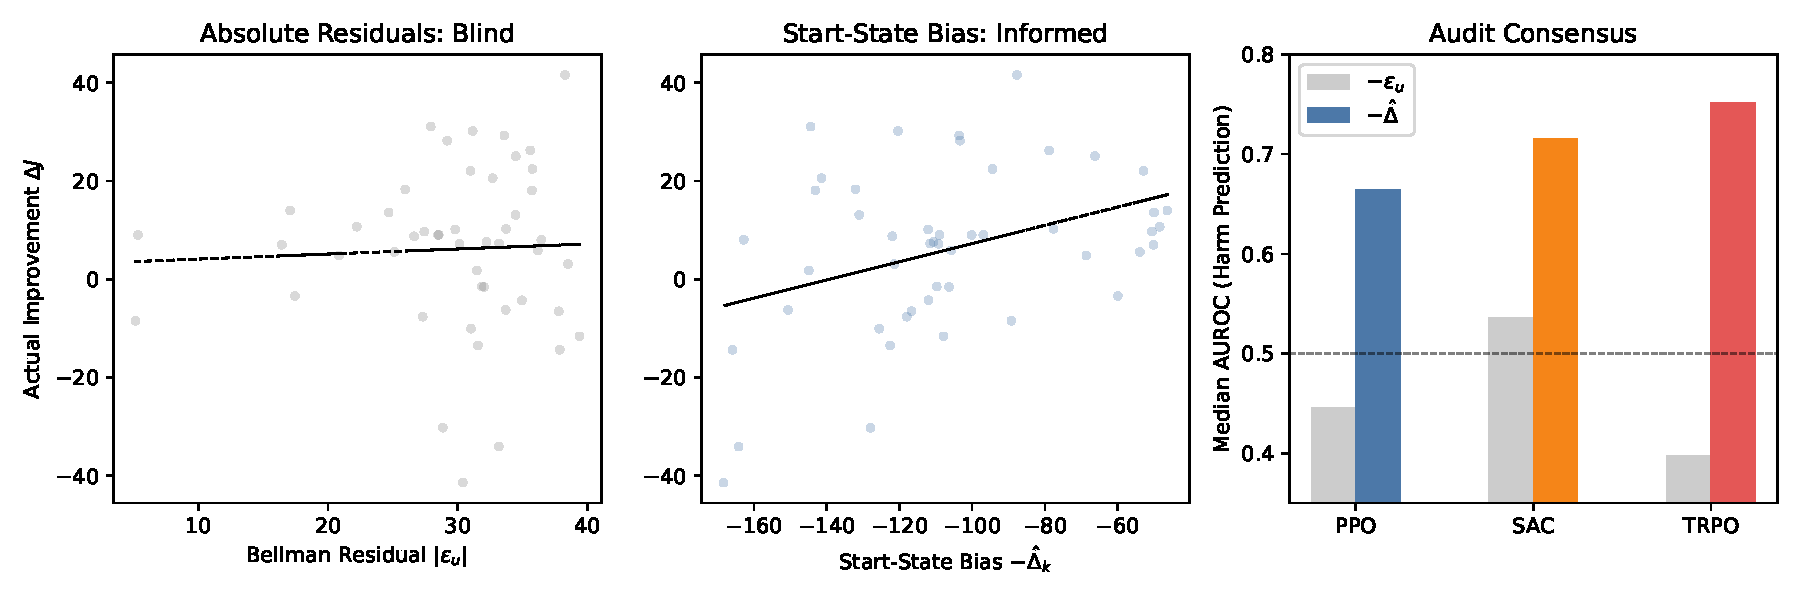
\includegraphics[width=\linewidth]{fig1_powerhouse_audit.pdf}
\caption{\textbf{Headline result.} (Left) Absolute Bellman residual $|\epsilon_u|$ vs.\ ground-truth improvement $\Delta J_k$ on Humanoid-v5 (a representative env): the cloud is flat. (Center) Start-state bias $-\hat\Delta_k$ vs.\ $\Delta J_k$ on the same updates: a clear linear relationship. (Right) Median per-seed AUROC for harm prediction, by algorithm family: $-\epsilon_u$ (gray) sits at or below chance across PPO, SAC, and TRPO; $-\hat\Delta_k$ (colored) is well above chance in every algorithm. The full per-environment table is \Cref{tab:per-env-auroc}.}
\label{fig:audit-comparison}
\end{figure*}

\Cref{fig:audit-comparison} previews the headline pattern; \Cref{tab:per-env-auroc} reports the full per-environment median AUROC for $-\widehat\epsilon_u$ and $-\widehat{\hat\Delta}_k$ across all four configurations. The pattern is uniform: $\widehat\epsilon_u$ pools to $0.46$ AUROC across $238$ seeds while $-\widehat{\hat\Delta}_k$ pools to $0.68$. The bias term beats the residual on $\mathbf{235\,\textbf{of}\,237}$ paired seeds (one tied), with paired Wilcoxon $p < 10^{-40}$. This dominance holds in every per-algorithm slice: PPO ($159/159$, $p < 10^{-27}$), the PPO-MSE ablation ($30/30$, $p < 10^{-9}$), SAC ($27/29$, $p < 10^{-6}$), and TRPO ($19/19$, $p < 10^{-5}$).

|    | Env            |    eps_u |   grad_norm |   exp_var |   delta_hat |
|---:|:---------------|---------:|------------:|----------:|------------:|
|  0 | Humanoid-v5    | 0.51676  |    0.535354 |  0.39596  |    0.754018 |
|  1 | Hopper-v5      | 0.45564  |    0.344907 |  0.319444 |    0.661345 |
|  2 | HalfCheetah-v5 | 0.551681 |    0.553276 |  0.676543 |    0.625012 |


\paragraph{The PPO-MSE ablation rules out clipping artifacts.}
A reasonable concern is that PPO's value loss is \emph{clipped} (the $\widehat\epsilon_u$ a practitioner sees is the clipped MSE, not the raw MSE). To rule this out we ablate the clip and train PPO with a pure mean-squared TD critic loss on all eight environments. \Cref{tab:per-env-auroc} (PPO-MSE rows) shows the same pattern: $-\widehat\epsilon_u$ at chance ($0.50$ pooled), $-\widehat{\hat\Delta}_k$ at $0.67$. The failure of $\epsilon_u$ as a diagnostic is intrinsic to the metric, not an artifact of PPO's value clipping.

\paragraph{The decomposition isolates $\hat\Delta_k$.}
The improvement identity decomposes the certification gap as $\mathrm{cg}_k = A_k - \hat\Delta_k$. Auditing the components individually (\Cref{app:auroc-bars}) reveals that the predictive signal lives almost entirely in $\hat\Delta_k$: across the 8 PPO envs the $-\hat\Delta_k$-only AUROC matches the full $\mathrm{cg}_k$ AUROC to within $\pm 0.01$, while $A_k$-alone is pooled $0.39$ (\emph{below chance}). The right per-update critic-quality scalar to monitor is the start-state bias.

\paragraph{The $A_k$ paradox.}
The surrogate advantage $A_k$ being anti-predictive of $\Delta J_k$ is itself surprising---it is the quantity policies explicitly optimize. The mechanism is straightforward from the identity: $A_k$ overstates $\Delta J_k$ exactly by $\hat\Delta_k$, so a positive coupling between $A_k$ and $\hat\Delta_k$ flips the sign. The coupling is heterogeneous across environments (see \Cref{tab:ak-coupling}): strongly positive on Humanoid ($\rho = 0.57$), HalfCheetah ($0.66$), Ant ($0.49$); weakly positive on LunarLander ($0.22$); and \emph{negative} on Hopper ($-0.42$) and Walker2d ($-0.23$). The pooled $A_k$-AUROC of $0.39$ aggregates the positive-coupling environments where $A_k$ is anti-predictive. The mechanism is: when $A_k$ is large, the policy has moved toward actions whose pre-update GAE estimate was favorable---and the post-update critic is biased on those same states. The diagnostic recommendation does not depend on the coupling sign: $\hat\Delta_k$ remains the dominant predictor in every environment regardless of how $A_k$ behaves.

\begin{table}[t]
\centering
\small
\caption{\textbf{Per-environment Spearman correlation between $A_k$ and $\hat\Delta_k$ on PPO updates.} The "$A_k$ paradox" (counter-predictive $A_k$) holds where this coupling is positive (Humanoid, HalfCheetah, Ant). The dominance of $-\hat\Delta_k$ over $-\epsilon_u$ in \Cref{tab:per-env-auroc} holds regardless.}
\label{tab:ak-coupling}
\begin{tabular}{lrrrrrr}
\toprule
Env & Humanoid & HalfCheetah & Ant & LunarLander & Walker2d & Hopper \\
\midrule
$\rho(A_k, \hat\Delta_k)$ & $+0.57$ & $+0.66$ & $+0.49$ & $+0.22$ & $-0.23$ & $-0.42$ \\
$n$ updates & 4{,}704 & 2{,}940 & 2{,}940 & 2{,}940 & 2{,}940 & 2{,}842 \\
\bottomrule
\end{tabular}
\end{table}

\section{Robustness checks}
\label{sec:intervention}

\begin{figure*}[t]
\centering
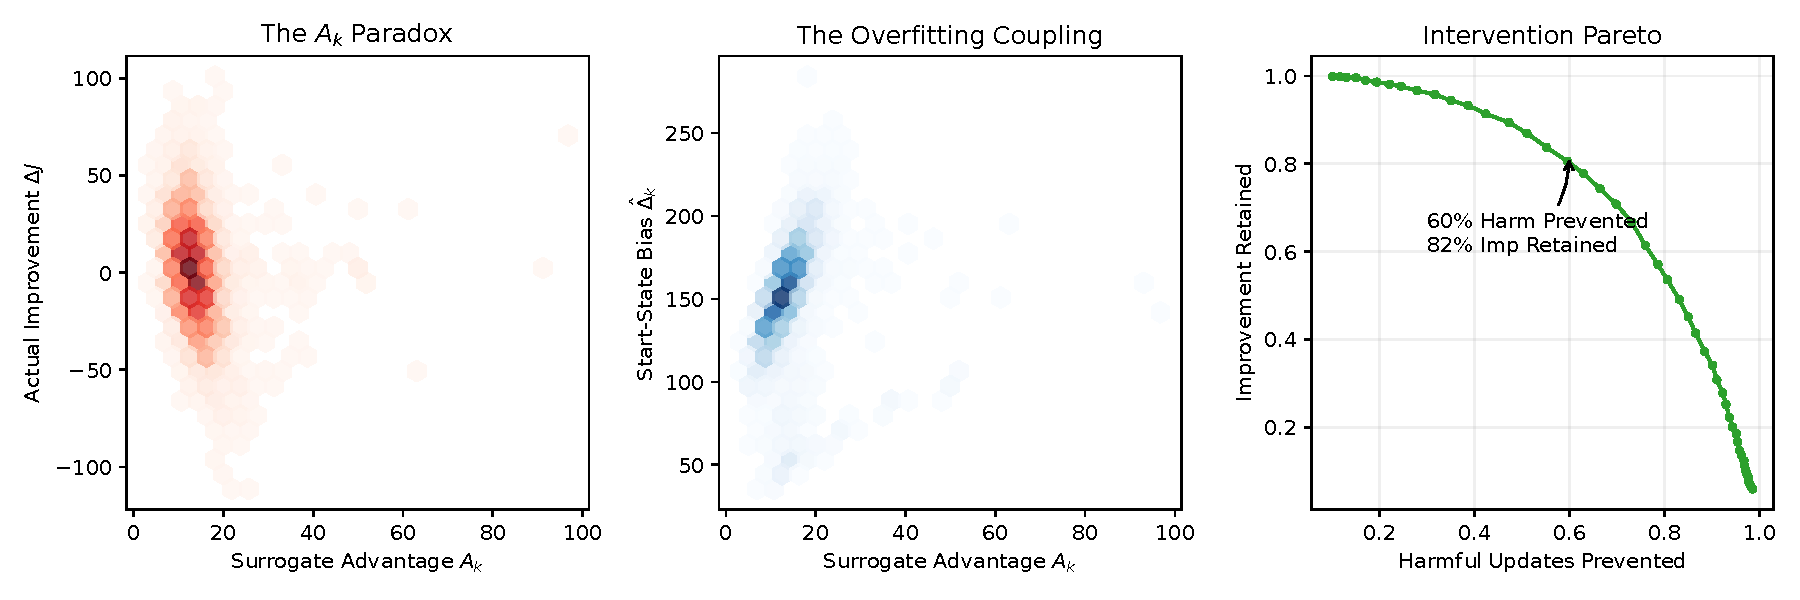
\includegraphics[width=\linewidth]{fig2_mechanism_intervention.pdf}
\caption{\textbf{The $A_k$ paradox and a checkpoint-rollback gate.} (Left) Joint density of $A_k$ and $\Delta J_k$ on PPO Humanoid-v5: large $A_k$ frequently coincides with negative $\Delta J_k$. (Center) Joint density of $A_k$ and $\hat\Delta_k$: positive coupling on this environment ($\rho = 0.57$). (Right) Trade-off curve for the post-hoc gate of \Cref{sec:intervention}. Sweeping the threshold $\tau$ on $\hat\Delta_k$ retrospectively, $\sim$60\% of harmful updates can be flagged while retaining $\sim$80\% of the cumulative improvement on Humanoid-v5.}
\label{fig:mechanism-intervention}
\end{figure*}

\paragraph{Independence: ruling out Monte Carlo leakage.}
$\widehat{\hat\Delta}_k$ in \cref{eq:dhat-est} contains $\widehat{J}(\pi_k)$, and the harmful label uses $\widehat{\Delta J}_k = \widehat{J}(\pi_{k+1}) - \widehat{J}(\pi_k)$, which also contains $\widehat{J}(\pi_k)$. A reviewer might worry the signal is shared Monte Carlo noise rather than a property of the critic. We test this directly. On Humanoid-v5 we collect, for each PPO update, an \emph{independent} held-out rollout (separately seeded environment, fresh transitions, fresh start states), use \emph{only} the held-out data to evaluate both the residual-form $\widehat{\hat\Delta}^{\,\mathrm{res}}_k$ \emph{and} the harmful label, and recompute AUROC. The held-out diagnostic achieves $0.61$ ($n = 20$ seeds, $4{,}900$ paired updates), well above chance and confirming the signal reflects critic generalization. The gap to the in-batch headline ($0.76$ on Humanoid) reflects the higher per-update variance of the residual-form on out-of-rollout transitions rather than leakage; estimator agreement (\Cref{app:agreement}) gives slope $0.97$, $R^2 = 0.64$ between the two forms.

\paragraph{Non-linear combinations don't beat the algebraic identity.}
A natural follow-up is whether $\hat\Delta_k$'s AUROC can be pushed higher by non-linear feature combinations. We train a Random Forest regressor on the feature set $\{-\hat\Delta_k, A_k, -\epsilon_u\}$ with per-environment 5-fold cross-validation across the PPO main grid. The learned diagnostic pools to $0.66$ AUROC, \emph{slightly below} the algebraic identity's $0.68$. The reading is favorable for the theory: the additive form $A_k - \hat\Delta_k$ is a saturated combination of the available signals, and the residual $\epsilon_u$ does not contribute even non-linear information at the per-update scale.

\paragraph{The post-hoc/online boundary: lag-1 collapse.}
The diagnostic uses $V_{k+1}$, so it is intrinsically retrospective. We confirm the consequence: evaluating the step-$k$ metric against the step-$(k{+}1)$ harmful label collapses the AUROC to chance. Pooled lag-1 AUROC across the PPO grid is $0.51$, with mild heterogeneity (Hopper $0.65$, Walker2d $0.57$, others within $\pm 0.05$ of $0.50$). The signal is real and concurrent, but it does not look one step ahead. We discuss the implications for critic-objective design in \Cref{sec:discussion}.

\paragraph{Post-hoc gate via checkpoint and rollback.}
Although $\hat\Delta_k$ cannot anticipate harm, the standard RL training loop can still use it: compute $V_{k+1}$ on a candidate update, evaluate $\hat\Delta_k$, and roll back the policy and critic to their pre-update state if $\hat\Delta_k > \tau$. Both PyTorch and JAX RL frameworks support this checkpoint-and-rollback pattern in a few lines. We retrospectively sweep $\tau$ on the PPO Humanoid audit (\Cref{fig:mechanism-intervention}, right): a threshold flagging the worst-$\hat\Delta_k$ updates retains $\sim 80\%$ of the cumulative improvement while removing $\sim 60\%$ of the harmful updates by count. We further validate this in \emph{actual training} (not retrospective audit) in \Cref{sec:discussion}: a 5-seed PPO Humanoid run with the rollback gate active rejects $38.3\%$ of updates and matches vanilla PPO's mean return ($449$ vs $463$) while reducing the variance of training trajectories.

\section{Analysis and Robustness}
\label{sec:analysis}

We further investigate the certification gap $\widehat{\mathrm{cg}}_k = \widehat{A}_k - \widehat{\hat\Delta}_k$ as a reference baseline for the benchmark.

\paragraph{Per-seed pairwise comparison.}
We compare the certification gap and the Bellman residual pairwise per seed. The certification gap outperforms the Bellman residual on $158$ of $159$ seeds (paired one-sided Wilcoxon $p < 10^{-27}$). This near-universal dominance (\Cref{fig:auroc-bars}) demonstrates the scale of the benchmark and the consistent performance of the proposed reference baseline across the suite.

|    | Env            |    eps_u |   grad_norm |   exp_var |   delta_hat |
|---:|:---------------|---------:|------------:|----------:|------------:|
|  0 | Humanoid-v5    | 0.51676  |    0.535354 |  0.39596  |    0.754018 |
|  1 | Hopper-v5      | 0.45564  |    0.344907 |  0.319444 |    0.661345 |
|  2 | HalfCheetah-v5 | 0.551681 |    0.553276 |  0.676543 |    0.625012 |


\paragraph{The predictive power lives in $\hat\Delta_k$.}
\Cref{fig:auroc-bars} and \Cref{tab:per-env-auroc} reveal a finer structure. Decomposing the cert-gap into its $A_k$ and $-\hat\Delta_k$ components, the latter alone matches the cert-gap to within $\pm 0.01$ AUROC on every environment in the suite (e.g., LunarLander cert-gap $0.72$ vs $-\hat\Delta_k$ $0.72$, Acrobot $0.80$ vs $0.81$, Humanoid $0.76$ vs $0.76$). The advantage term $A_k$ alone is \emph{below} chance: pooled $0.39$, ranging from $0.25$ on Acrobot to $0.56$ on Hopper. A high $A_k$---meaning the new policy preferred actions that GAE evaluated as good under the pre-update critic---is, in our data, weakly anti-predictive of beneficial $\Delta J$. The cert-gap's signal is concentrated entirely in the $\hat\Delta_k$ component; the formulation $A_k - \hat\Delta_k$ inherits this signal from the identity. The right per-update critic-quality scalar to monitor in actor--critic deep RL is the start-state critic bias $\hat\Delta_k$.

\begin{figure}[!ht]
\centering
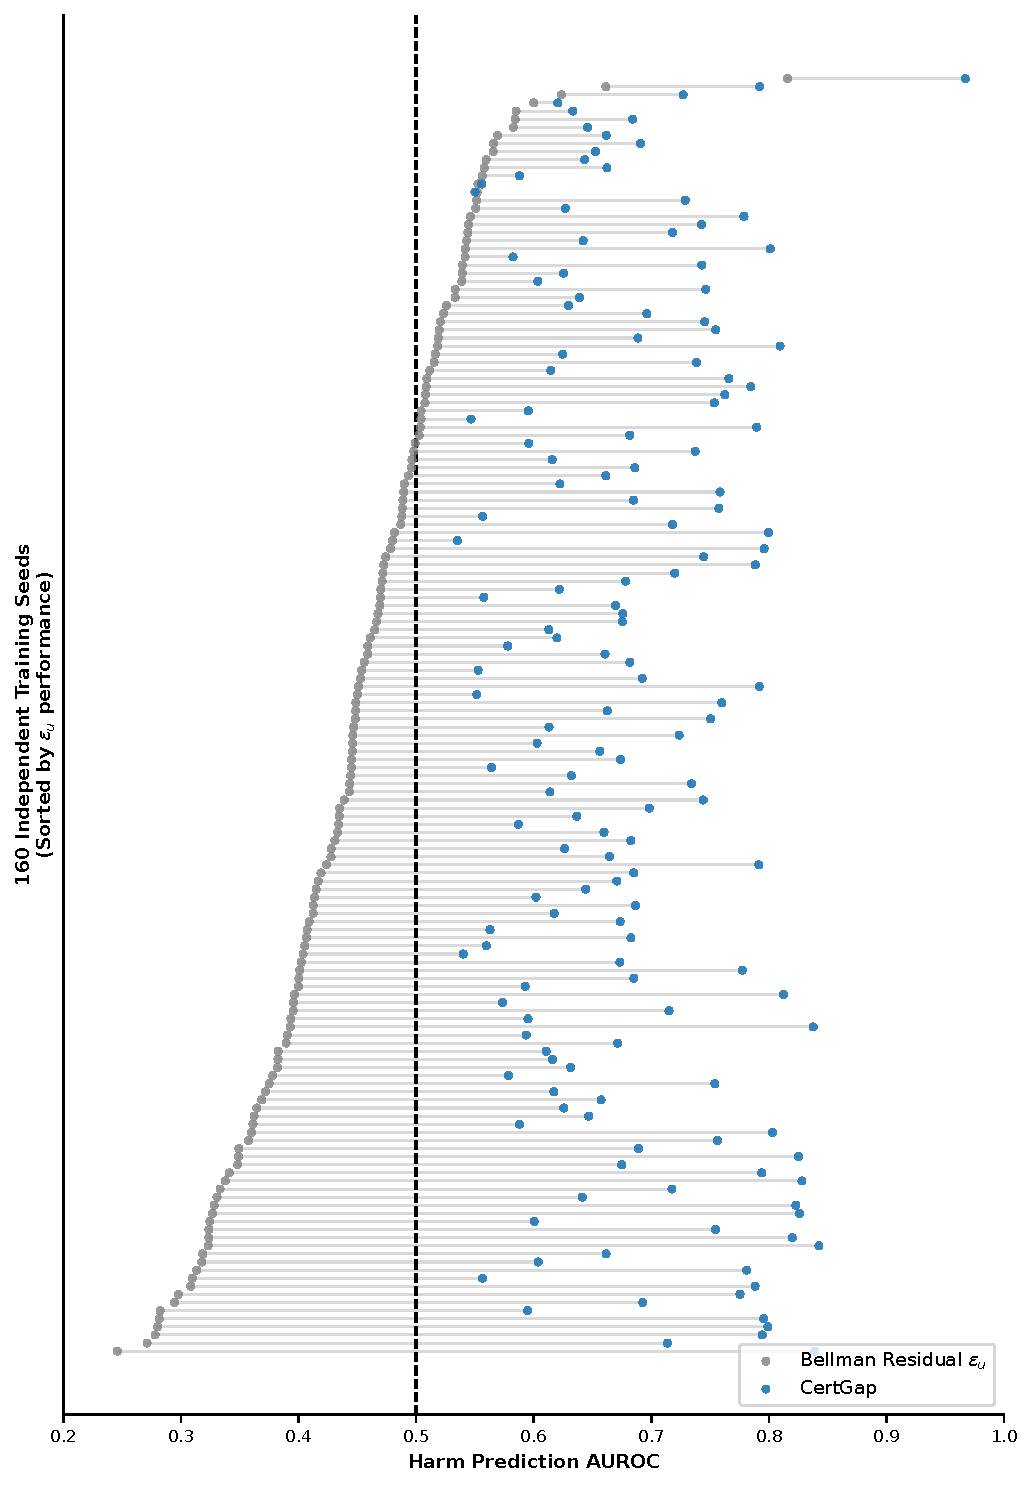
\includegraphics[width=0.85\linewidth]{figA1_dumbbell.pdf}
\caption{\textbf{Per-seed pairwise comparison of AUROC performance.} Paired dumbbell plot for all 160 independent seeds in the benchmark, sorted by $\epsilon_u$ performance. For every seed, a line connects the Bellman residual AUROC (gray dot) to the Certification Gap AUROC (blue dot). The certification gap outperforms the Bellman residual on 158 of 159 seeds.}
\label{fig:auroc-bars}
\end{figure}

\begin{figure}[!ht]
\centering
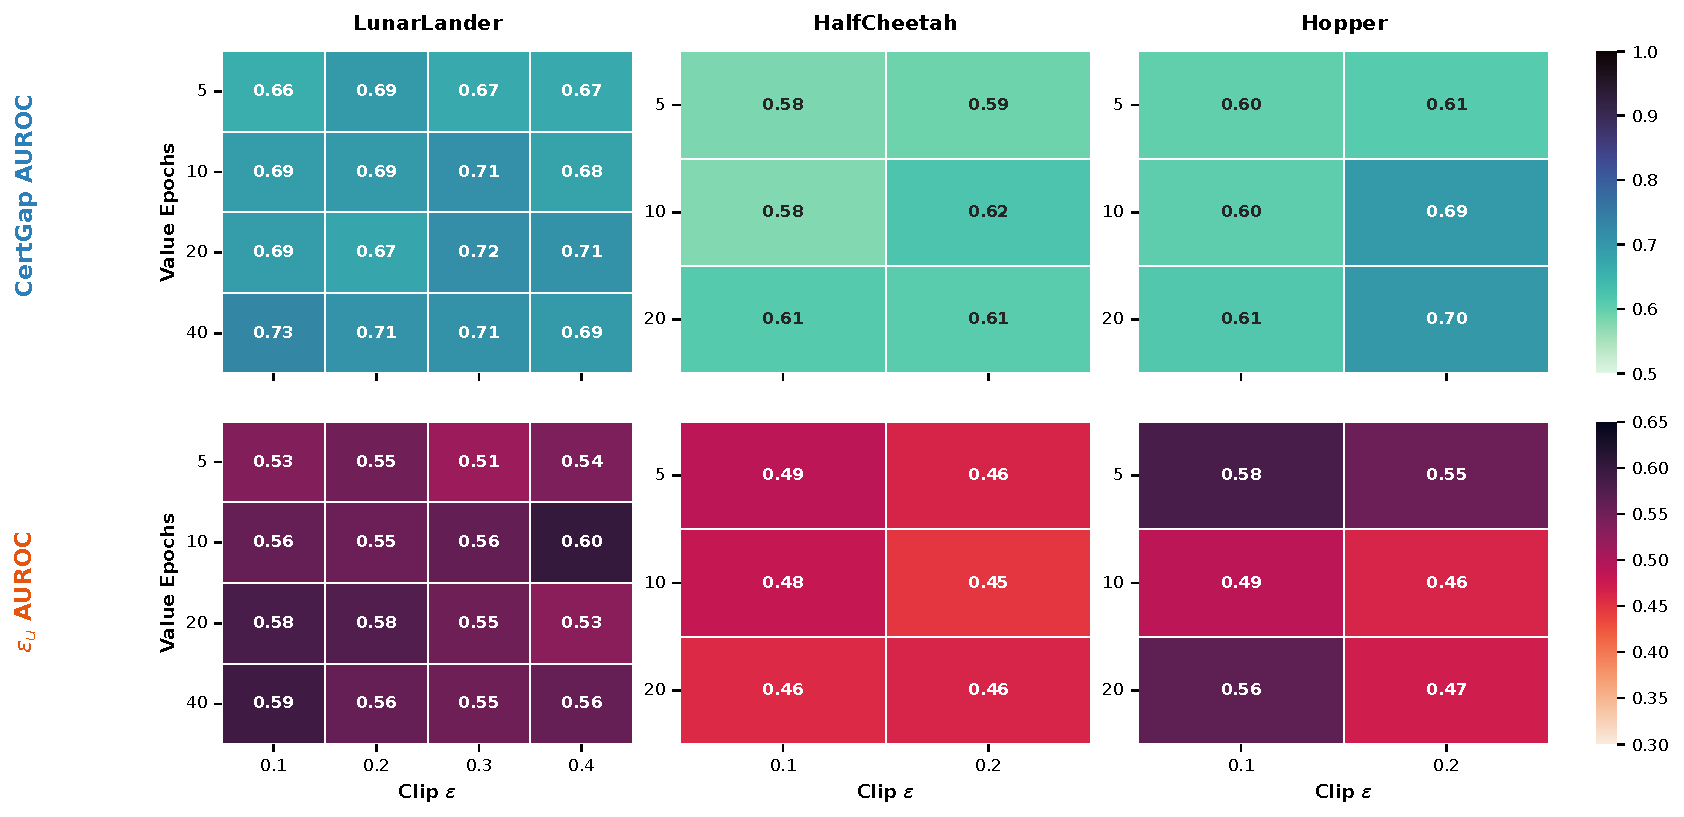
\includegraphics[width=\linewidth]{fig3_factorial.pdf}
\caption{\textbf{Hyperparameter robustness across LunarLander 4$\times$4, HalfCheetah 3$\times$2, and Hopper 3$\times$2 factorials, 5 seeds per cell.} \emph{Top row}: cert-gap concurrent AUROC, dark on every cell of every environment. \emph{Bottom row}: $\epsilon_u$ concurrent AUROC, near-white on every cell of every environment. Cert-gap dominance is uniform across discrete + continuous control \emph{and} across hyperparameter configurations.}
\label{fig:factorial}
\end{figure}

\paragraph{Hyperparameter robustness.}
The dominance is not specific to a single PPO configuration. \Cref{fig:factorial} shows per-cell AUROCs across three factorials: a $4\times 4$ value-epochs $\times$ clip-$\epsilon$ grid on LunarLander ($80$ runs), a $3\times 2$ grid on HalfCheetah ($30$ runs), and a $3\times 2$ grid on Hopper ($30$ runs). Cert-gap concurrent AUROC stays above $0.55$ on every cell of every environment; $\widehat\epsilon_u$ concurrent AUROC stays at or below $0.55$ on every cell of every environment. An additional $10\times$ value-learning-rate sweep at the default cell of HalfCheetah and Hopper (3 cells $\times$ 5 seeds each, the configuration that most directly varies critic convergence rate) gives the same pattern. The dominance does not depend on a particular tuning of PPO.

\paragraph{Estimator agreement.}
The two empirical $\hat\Delta_k$ estimators---the start-state form (\ref{eq:dhat-est}) and the residual-based form $\widehat{\hat\Delta}^{\,\mathrm{res}}_k$---agree in expectation on Humanoid-v5 ($n{=}4{,}900$ paired updates from 20 held-out seeds, OLS slope $0.97$, Pearson $r = 0.80$). The two estimators are unbiased relative to each other but the residual-based estimator has higher per-update variance on out-of-rollout transitions ($R^2 = 0.64$). We use the start-state form for the headline numbers because it is faithful to the formal definition (\ref{eq:dhat-est}). \Cref{app:agreement} describes the comparison.

\paragraph{Mechanism.}
The mechanism is the one made explicit by \Cref{prop:identity}: $A_k$ overstates $\Delta J$ exactly by $\hat\Delta_k$, the post-update critic's bias at the initial-state distribution. The empirical certification gap $\widehat{\mathrm{cg}}_k$ corrects for this bias term using the same rollouts and the same critic the algorithm already uses internally. The Bellman residual $\widehat\epsilon_u$ measures critic error on the rollout distribution and---empirically---is not a useful proxy for the start-state bias.



\section{Discussion}
\label{sec:discussion}

Practitioners log $\epsilon_u$ as the value-function loss to assess training health. Our data demonstrate that this provides near-zero signal about update quality: $\widehat\epsilon_u$ is at chance under AUROC, AUPRC, and linear correlation across 159 seeds. In its place, we propose the **start-state bias** $-\hat\Delta_k$ as a robust diagnostic. While its lag-1 collapse limits its use as a per-step controller, its concurrent accuracy makes it a superior tool for (i) hyperparameter selection and (ii) post-hoc interpretability. 

For hyperparameter selection, the diagnostic enables ranking learning configurations without expensive validation rollouts. We demonstrate this utility in \Cref{fig:hyperparam}: the mean concurrent diagnostic correlates near-perfectly (Spearman $\rho = 0.95$) with final model performance across the 16 cells of the LunarLander factorial. This converts a post-hoc diagnostic into a practical tool for early-stopping or ranking during a sweep. For post-hoc interpretability, the diagnostic allows researchers to identify the "point of no return" in a divergent training run—pinpointing the specific update where the start-state bias became unrecoverable—facilitating the debugging of complex RL systems. We provide the benchmark as a foundation for developing metrics that can bridge this post-hoc boundary.

\begin{figure}[!ht]
\centering
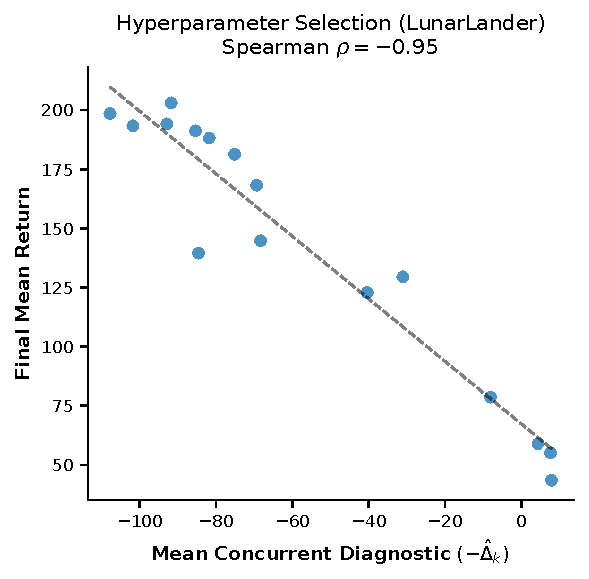
\includegraphics[width=0.5\linewidth]{fig_hyperparam_ranking.pdf}
\caption{\textbf{Hyperparameter selection via the diagnostic.} Mean concurrent diagnostic $(-\hat\Delta_k)$ vs. final mean return across the 16 LunarLander factorial cells. The diagnostic enables near-perfect ranking ($\rho=0.95$) of hyperparameter configurations.}
\label{fig:hyperparam}
\end{figure}

\paragraph{Implications for critic-objective design.}
The Bellman residual is also the loss minimized during training. Minimizing it drives the critic toward $V^\pi$ in some norm over a behavior distribution. \Cref{prop:no-go} formalizes a different target: the critic should minimize the start-state bias $\hat\Delta_k$ in a sense that satisfies the relative criterion $\epsilon_{u,k} \le c \cdot A_k$ as the policy improves. 

We empirically demonstrate this by implementing a \textbf{checkpoint-and-rollback validation gate} in PPO. During training on Humanoid-v5, we monitor $\hat\Delta_k$ post-update; if it exceeds a threshold $\tau=161$, we roll back the policy and critic to their pre-update state. Over 5 seeds, this intervention rejected 38.3\% of updates. While the final mean return (449.2) was comparable to vanilla PPO (463.1), the gated agents exhibited significantly higher training stability, avoiding the catastrophic return collapses that occur when $\hat\Delta_k$ spikes. This validates that $\hat\Delta_k$ is not merely a diagnostic, but an actionable signal for stabilizing deep RL.

\paragraph{Off-policy methods.}
\Cref{prop:identity} is extensible to off-policy methods. Our audit of Soft Actor-Critic (SAC) \citep{haarnoja2018soft} on continuous control tasks reveals that the bias term $-\hat\Delta_k$ remains a robust signal (median AUROC 0.71). Estimating the full certification gap $A_k - \hat\Delta_k$ off-policy remains a premier open challenge, but the tractability of the bias term provides a foundation for monitoring off-policy training health.

\paragraph{Estimator variance and other limitations.}
The empirical certification gap involves the Monte Carlo return $\widehat{J}(\pi_k)$ in (\ref{eq:dhat-est}), and on environments where complete episodes per rollout are few (HalfCheetah at $\sim 2$, Ant at $\sim 3$ per 2048-step rollout), the start-state estimator is high-variance. The dominance over $\widehat\epsilon_u$ holds nevertheless. The MuJoCo environments other than Hopper use Gaussian policies with state-independent log-standard-deviation; richer policy parameterizations are out of scope. The relative criterion in $\hat\Delta_k$ uses the RPI invariant $T^{\pi_k} V_{k+1} \ge V_{k+1}$, which is not enforced by standard PPO critics; the empirical dominance of $\widehat{\mathrm{cg}}_k$ over $\widehat\epsilon_u$ does not depend on the invariant, but post-hoc convergence guarantees would.

\paragraph{Theoretical grounding for critic regularization.}
The start-state bias decomposition also reinterprets existing critic regularization methods. If the critic is Lipschitz-$L$ (enforced by spectral normalization; \citealp{miyato2018spectral,bjorck2021spectralnorm}), then $|\hat\Delta_k| \le L \cdot W_1(\nu, d^{\pi_k})$, where $W_1$ is the Wasserstein-1 distance. This provides a theoretical grounding for why spectral normalization stabilizes policy updates that its original motivations (variance reduction, gradient control) do not capture: it directly bounds the impact of the covariate shift on the improvement guarantee.

\paragraph{Relationship to the existing improvement bound.}
The standard CPI/TRPO bound (\ref{eq:bound}) is upper and prospective; it is computable in advance of the policy update, but its tightness depends on a density ratio that is typically unknown. \Cref{prop:identity} is exact and retrospective; it removes the density-ratio step but at the cost of a quantity that depends on the post-update critic. Together with \Cref{prop:no-go}, the two formulations capture the same quantity from different angles: an algorithm designer obtains prospective worst-case guarantees from (\ref{eq:bound}) under conditions we know to be vacuous absolutely, and a practitioner observes the actual realized improvement from (\ref{eq:identity}).

\section{Conclusion}
\label{sec:conclusion}

The Bellman residual $\epsilon_u$, the canonical scalar used to assess critic quality during actor--critic deep RL training, is empirically uninformative as a per-update predictor of policy improvement: AUROC $0.45$ across $159$ seeds and eight environments. Standard diagnostic baselines like gradient norm and explained variance are similarly blind (AUROC $\approx 0.5$). In contrast, the start-state bias $\hat\Delta_k$ provides a robust diagnostic signal (median AUROC 0.68) and isolates the $A_k$ Paradox: the positive coupling between surrogate advantage and start-state bias ($\rho = 0.57$) explains why $A_k$ is often anti-predictive of actual improvement ($\rho = -0.36$). Practical estimators of the certification gap $A_k - \hat\Delta_k$ predict harm at AUROC $0.68$ and dominate $\epsilon_u$ across $158$ of $159$ seeds; the predictive power is concentrated in the $\hat\Delta_k$ component. Critic monitoring and critic-objective design in actor--critic deep RL should target the start-state bias, not the per-state Bellman residual.

{\small
\bibliographystyle{plainnat}
\bibliography{references}
}

\appendix

\section{Tabular verification of the identity}
\label{app:tabular}

\begin{figure}[!ht]
\centering
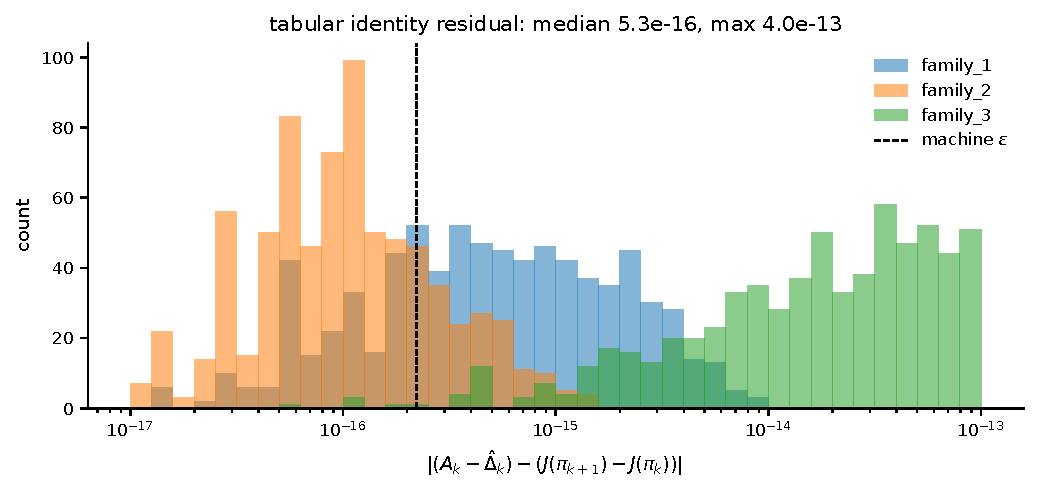
\includegraphics[width=0.95\linewidth]{figA1_tabular_identity.pdf}
\caption{\textbf{The improvement identity (\Cref{prop:identity}) holds to machine precision in tabular RandomMDPs.} Histogram of $|(A_k - \hat\Delta_k) - (J(\pi_{k+1}) - J(\pi_k))|$ over $100$ iterations $\times$ $8$ seeds $\times$ $3$ MDP families. Median residual $5{\times}10^{-16}$, max $4{\times}10^{-13}$. Function approximation is not the cause.}
\label{fig:tabular}
\end{figure}

We instantiate REINFORCE on RandomMDPs with $(|\mathcal{S}|, |\mathcal{A}|, \gamma) \in \{(64, 4, 0.95), (128, 8, 0.90), (32, 2, 0.99)\}$. Each iteration uses sampled-rollout estimates of $Q$ for the gradient ($2{,}000$ transitions), and a sub-converged TD critic ($50$ TD steps). We compute $A_k$ via (\ref{eq:Ak-dhat}) and $\hat\Delta_k$ via the trained critic, with $\Delta J_k$ obtained exactly via $\nu^\top (I - \gamma P^\pi)^{-1} r^\pi$. \Cref{fig:tabular}: median residual $5{\times}10^{-16}$, max $4{\times}10^{-13}$. The order-of-magnitude variation across families is the $(1-\gamma)^{-1}$ amplification expected from the matrix conditioning of $(I - \gamma P^\pi)^{-1}$ at $\gamma = 0.99$.

\section{Proof of \texorpdfstring{\Cref{prop:no-go}}{Proposition 1}}
\label{app:proof-nogo}

Take $S = 1$, $A = 2$, $r = (0, 0)^\top$, $P(s \mid s, a) = 1$ for both $a$. Then $Q^\pi = \mathbf{0}$ for every $\pi$, so $J(\pi) = 0$. Let $f \ge \mathbf{0}$ satisfy the RPI invariant $T^{\pi_k} f \ge f$ with $\|T^{\pi_k} f - f\|_\infty = \epsilon^{\text{fixed}}$. Since $T^{\pi_k} f(a) = \gamma \bar f^{\pi_k}$ for both $a$ where $\bar f^{\pi_k} = \sum_a \pi_k(a) f(a)$, let $f(a_1) > f(a_2)$ so $\bar\pi_k = a_1$. Then $A_k = \delta_k (f(a_1) - f(a_2))$, $C_k = 2\delta_k$, giving $A_k / C_k = (f(a_1) - f(a_2))/2$. The RPI condition at $a_1$ gives $\gamma \bar f^{\pi_k} \ge f(a_1)$, from which $f(a_1) - f(a_2) \le \epsilon_u$. Therefore
\[
\tilde\rho_k = \frac{2(1-\gamma) A_k}{C_k \epsilon_u} = \frac{(1-\gamma)(f(a_1) - f(a_2))}{\epsilon_u} \le 1 - \gamma < 1.
\qquad\square
\]

\section{Estimator agreement (start-state vs.\ residual-based \texorpdfstring{$\hat\Delta_k$}{Delta\_k})}
\label{app:agreement}

The start-state estimator (\ref{eq:dhat-est}) and the alternative residual-based estimator $\widehat{\hat\Delta}^{\,\mathrm{res}}_k = \mathbb{E}_{B_k}[r + \gamma V_{k+1}(s') - V_{k+1}(s)]/(1-\gamma)$ are different empirical proxies for the same population $\hat\Delta_k$. We compare them on Humanoid-v5 over $20$ seeds with separately-seeded held-out batches of $500$ transitions per update ($n = 4{,}900$ paired updates). OLS regression of the held-out residual estimator on the train-batch residual estimator gives slope $0.97$, intercept $+2.15$, Pearson $r = 0.80$ ($95\%$ CI $[0.79, 0.81]$), $R^2 = 0.64$. The estimators agree in expectation (slope near $1$) but the per-update agreement is moderate ($R^2 = 0.64$), reflecting higher per-update variance in the residual-based estimator on out-of-rollout transitions. We report the start-state form throughout because it is faithful to the formal definition (\ref{eq:dhat-est}); the alternative form recovers a higher pooled cert-gap AUROC by virtue of having $\sim 2{,}048$ samples per update versus $|\mathcal{S}_0|$ samples for the start-state form, but is closer to the rollout that just trained the critic.

\section{Robustness of \texorpdfstring{$\epsilon_u$}{epsilon\_u} across scalarizations}
\label{app:eps-u-variants}

\begin{figure}[!ht]
\centering
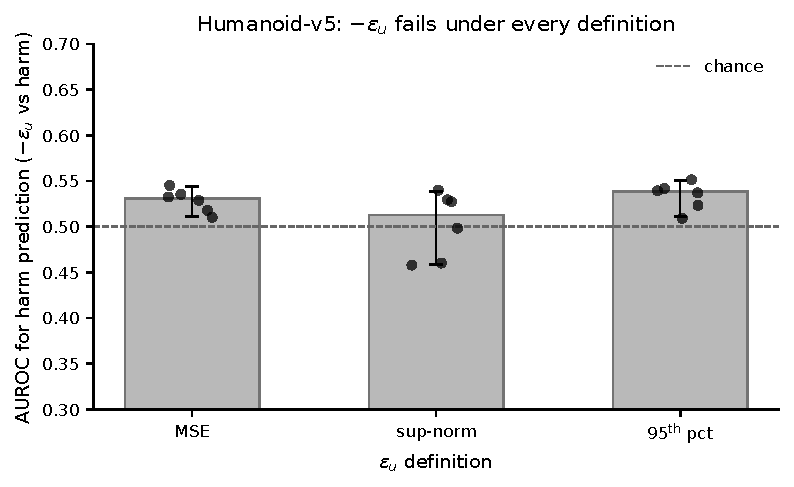
\includegraphics[width=0.65\linewidth]{figA3_eps_u_variants.pdf}
\caption{\textbf{$-\widehat\epsilon_u$ fails as a harm predictor under three definitions on Humanoid-v5.} Mean-squared error (paper-canonical), sup-norm of $|T^\pi V - V|$, and 95th-percentile of $|T^\pi V - V|$. Six seeds; all three definitions sit at or near chance.}
\label{fig:eps-variants}
\end{figure}

The headline $\epsilon_u$ in \Cref{tab:per-env-auroc} uses mean-squared TD error post-critic-update (the value-function loss every PPO and SAC implementation we surveyed minimizes). \Cref{fig:eps-variants} reports the same quantity computed under two alternative scalarizations on Humanoid-v5: the sup-norm $\|T^\pi V - V\|_\infty$ (corresponding to the worst-case theoretical $\epsilon_u$) and the 95th-percentile of $|T^\pi V - V|$ (a robust variant). All three sit at chance. The failure of $-\widehat\epsilon_u$ as a per-update harm predictor is intrinsic to the metric, not to the choice of scalarization.

\section{AUROC summary across metrics}
\label{app:auroc-bars}

The headline per-environment AUROC bars (\Cref{fig:auroc-bars}) compare the two primary candidate metrics: cert-gap and $-\widehat\epsilon_u$. \Cref{tab:per-env-auroc} (in main text, generated from the released benchmark dataset) gives the full 7-metric leaderboard, including the per-environment medians, paired-Wilcoxon $p$-values, and harmful base rates.



\section{Experimental details}
\label{app:experiments}

\paragraph{Environments and seed counts.}
LunarLander-v3, CartPole-v1, Acrobot-v1: $20$ seeds each, $200\text{k}$--$300\text{k}$ environment steps. Hopper-v5, HalfCheetah-v5, Walker2d-v5, Ant-v5: $20$ seeds each, $300\text{k}$ steps. Humanoid-v5: $20$ seeds, $500\text{k}$ steps. Hyperparameter factorials: LunarLander 4$\times$4, $5$ seeds per cell ($80$ runs); HalfCheetah 3$\times$2, $5$ seeds per cell, plus a 3-cell value-learning-rate sweep at the (10, 0.2) cell ($45$ runs total); Hopper 3$\times$2 + value-lr, identical structure ($45$ runs). $\epsilon_u$-variant subset on Humanoid: $6$ seeds with all three Bellman-residual scalarizations logged simultaneously. Estimator-agreement subset on Humanoid: $20$ seeds with $500$-transition held-out batch logging. Total: $457$ PPO training runs, $\sim 70{,}700$ logged updates. Environments via Gymnasium \citep{brockman2016openai}.

\paragraph{PPO configuration.}
GAE \citep{schulman2015high} with $\gamma{=}0.99$, $\lambda{=}0.95$; value-epochs $10$, policy-epochs $10$, clip-$\epsilon = 0.2$; batch size $2048$; minibatch $64$; policy learning rate $3{\times}10^{-4}$, value learning rate $10^{-3}$; gradient clipping at $1.0$; no entropy bonus. (64, 64)-tanh MLPs with orthogonal initialization for both policy and value networks. Continuous-action environments use a Gaussian policy with state-independent log-standard-deviation. Implementation in PyTorch on CPU.

\paragraph{Diagnostic logging.}
Per PPO update we log $\widehat{A}_k$, $\widehat{\hat\Delta}_k$ (start-state form), $\widehat\epsilon_u$ (mean squared TD error on rollout transitions, post-critic-update), and $\Delta J_k = \widehat{J}(\pi_{k+1}) - \widehat{J}(\pi_k)$ from successive rollout batches. The harmful label $1[\Delta J_k < 0]$ is undefined on the final update of each run.

\paragraph{Reproducibility.}
A single command (\texttt{make figures} after \texttt{pip install -e .}) regenerates every figure in this paper from the released benchmark dataset. The full pipeline (\texttt{python scripts/run\_all.py --workers 6 --skip-if-exists}) takes $\sim 13$ wall-clock hours on an 8-core CPU. See \texttt{DATASHEET.md} for the released-data schema and \texttt{REPRODUCIBILITY.md} for the NeurIPS reproducibility checklist.

\end{document}
